% !TEX TS-program = pdflatex
% !TEX encoding = UTF-8 Unicode
%
% -----------------------------------------------------
% LaTeX-Vorlage
%
% LABREPORT v1
% von Markus Kn�sel frei nach KOMA-Script-Klassen
% -----------------------------------------------------
%
\documentclass[11pt,titlepage]{scrartcl}		% Schriftgr��e festlegen, standard 10pt 
%
\usepackage[latin1]{inputenc}				% input encoding f�r vim/utf8/Umlaute
\usepackage[T1]{fontenc}
\usepackage{lmodern} 
%
% -----------------------------------------------------
\usepackage{geometry} 					% legt die Blattgr��e und Randabst�nde fest
\geometry{a4paper}
\geometry{margin=3cm,top=2.5cm,bottom=2.5cm}
%
%
%
%
%
%
% -----------------------------------------------------
\usepackage{graphicx} 					% support the \includegraphics command and options
\usepackage[parfill]{parskip}				% Activate to begin paragraphs with an empty line rather than an indent
\usepackage{booktabs}					% for much better looking tables
%\usepackage{array}					% for better arrays (eg matrices) in maths
\usepackage{paralist}					% very flexible & customisable lists (eg. enumerate/itemize, etc.)
\usepackage{verbatim}					% adds environment for commenting out blocks of text & for better verbatim
\usepackage{subfig}					% make it possible to include more than one captioned figure/table in a single float
\usepackage{color}
\usepackage[german]{babel}
\usepackage{units}
\usepackage[onehalfspacing]{setspace}
\usepackage{amsmath,amsfonts,amssymb}
\usepackage{icomma,units}
\usepackage{enumerate}
\usepackage[margin=10pt,font=small,labelfont=bf,labelsep=endash]{caption}
\usepackage{chemmacros}
\usepackage{chemfig}
\usepackage{PSTricks}
\usepackage{epstopdf}
\usepackage[ngerman=ngerman-x-latest]{hyphsubst}
\usepackage{pgfplots}
\usepackage{pgfplotstable}
%
%
%
%
% ---------- HEADERS & FOOTERS ------------------------
\usepackage{fancyhdr} % This should be set AFTER setting up the page geometry
\pagestyle{fancy} % options: empty , plain , fancy
%\renewcommand{\headrulewidth}{0pt} % customise the layout...
\lhead{Markus Kn�sel}\chead{}\rhead{\textsc{Physikalische Chemie II}}
%\lfoot{}\cfoot{\thepage}\rfoot{}
%
%
%
%
% ---------- SECTION TITLE APPEARANCE -----------------
\usepackage{sectsty}
\definecolor{cyan}{RGB}{30,103,182}      % hellgruener Rahmen
\allsectionsfont{\mdseries\upshape\textcolor{cyan}} % (See the fntguide.pdf for font help)
%
%
%
%
% ---------- ToC (table of contents) APPEARANCE -------
\usepackage[nottoc,notlof,notlot]{tocbibind} % Put the bibliography in the ToC
\usepackage[titles,subfigure]{tocloft} % Alter the style of the Table of Contents
% \renewcommand{\cftsecfont}{\rmfamily\mdseries\upshape}
% \renewcommand{\cftsecpagefont}{\rmfamily\mdseries\upshape} % No bold!
%
%
%
%
% ---------- TITLEPAGE DETAILS ------------------------
\addtokomafont{subject}{\sc}
\setkomafont{title}{\normalfont}
	\subject{Nachweis der im Daniell-Element ablaufenden Reaktionen}
	\title{Versuchsprotokoll}
	\subtitle{3812 - Praktikum Physikalische Chemie II}
	\author{\normalfont Markus Kn�sel \\ Matrikelnr. 23 94 86 }
	\date{durchgef�hrt am 30.11.14} % Activate to display a given date or no date (if empty),
\publishers{\normalsize 
\includegraphics[width=4cm]{unilogo} \\ Fachbereich IV \\ Abteilung f�r Chemie}
%
%
%
%
% ---------- DOCUMENT ---------------------------------
%
\newtagform{equation}{\{}{\}}
\usetagform{equation}
%
\begin{document}
	\maketitle
	\tableofcontents
	\newpage
%
% ------ Equation/Reaction Counter ---------
\RenewEnviron{reaction}{\begin{equation} \expandafter \ch\expandafter {\BODY} \end{equation}}
\RenewEnviron{reaction*}{\begin{equation*}\expandafter \ch\expandafter{\BODY}\end{equation*}}
\RenewEnviron{reactions}{\begin{align}\expandafter\ch\expandafter{\BODY}\end{align}}
\RenewEnviron{reactions*}{\begin{align*}\expandafter\ch\expandafter{\BODY}\end{align*}}
%
%\NewChemState\ElPot[subscript-left=false,exponent=]{E}{\volt}


%	
%
%
%% \section*{\abstractname}
%% Blabla
%
\section{Theoretische Grundlagen}
In diesem Versuch sollen die einzelnen Halbzellenreaktionen des Daniell-Elements nachgewiesen werden. Wie im vorherigen Versuch ausf�hrlich beschrieben, lautet die Gesamtreaktion
\\[5ex]
\begin{center}
\ch{
%	\vspace{14mm}
	"\OX{o1,\ox{+2,Cu}}\pch[2]"  + "\OX{r1,\ox{0,Zn}}"
	->
	"\OX{o2,\ox{0,Cu}}"  + "\OX{r2,\ox{+2,Zn}}\pch[2]"
}
\redox(o1,o2)[draw=red,->][3.33]{\small Red.: $+ 2\el$}
\redox(r1,r2)[draw=blue,->]{\small Ox.: $- 2\el$}
\label{1}
\end{center}
Um nun die Teilreaktionen nachweisen zu k�nnen, werden nicht mehr Kupfer- und Zinnelektroden und ihre Salzl�sungen verwendet, sondern die Apparatur wir im Folgendem beschrieben aufgebaut.
%
%
\section{Versuchsdurchf�hrung}
%
\begin{figure}[h]
	\centering
	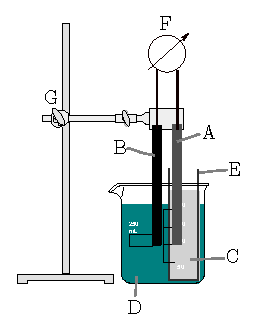
\includegraphics{aufbau.eps}
	\caption{Versuchsaufbau mit Zinkblech (A), Graphitelektrode (B), \ch{KNO3}-L�sung (1 \unitfrac{mol}{l} (C), \ch{CuSO4}-L�sung (1 \unitfrac{mol}{l} (D), Tonzelle (E), Multimeter (F) und Stativ mit Klemmen und Elektrodenhalter (G)}
	\label{fig:aufbau}
\end{figure}
%
\begin{singlespace}
	\small\underline{Ger�te:}~Tonzelle, Becherglas 250~ml, Multimeter, Verbindungskabel, Zinkblech, Kohleelektrode, 2 Krokodilklemmen\\[1ex]
	\underline{Chemikalien:}~\ch{CuSO4}-L�sung (1 \unitfrac{mol}{l}), \ch{KNO3}-L�sung (1 \unitfrac{mol}{l}), \ch{K3[Fe(CN)6]}-L�sung (2\%)\\[1ex]
\end{singlespace}
%
Die Apparatur wird wie nach Abbildung~\ref{fig:aufbau} aufgebaut. Das Zinkblech wird vor und nach Versuchsdurchf�hrung gewogen. Zu beachten ist, da� die \ch{KNO3}-L�sung in der Tonzelle h�her steht als die \ch{CuSO4}-L�sung im Becherglas. Nach Messen der Zellspannung wird das Element f�r ungef�hr 30 Minuten mit einem Verbindungskabel kurzgeschlossen. Anschlie�end wird das Zinkblech abgesp�lt und gewogen. Die Messwerte sind in Tabelle \ref{tab:gewicht} aufgef�hrt.
%
\section{Auswertung}
Die mit Hilfe des Multimeter bestimmte elektromotorische Kraft des galvanischen Elements betr�gt
\begin{equation*}
	\Delta E = 1,29~\si{\volt}.
\end{equation*}
%
Die Zinkelektrode hat messbar an Masse zugenommen. Wie auch im Daniell-Element findet am Zinkblech die Oxidation statt, es stellt hier die Anode dar. An der Kohleelektrode hingegen werden Kupferionen zu elementarem Kupfer reduziert, es handelt sich im die Kathodenreaktion. Durch die Wand der Tonzelle diffundieren die \ch{NO3}- und \ch{SO4}-Ionen. Nach einigen Minuten ist ein kupferfarbener Schimmer an der Elektrode zu erkennen, nach 30 Minuten hat sie einen deutlich erkennbaren Kupfer�berzug. Um das in L�sung gegangene Zink in der \ch{KNO3}-L�sung nachzuweisen, entnimmt man einige Milliliter der Anodenfl�sigkeit und f�gt wenige Tropfen einer \ch{K3[Fe(CN)6]}-L�sung hinzu. Es entsteht ein braungelber Niederschlag, der in verd�nnten S�uren schwer l�slich ist. (\textsc{Jander Blasius}, S. 194)
\begin{reaction}
	3 Zn\pch[2] + 2 [Fe(CN)6]\mch[3] -> Zn3[Fe(CN)6]2
\end{reaction}
In diesem Versuch ist das abgeschiedene elementare Kupfer eindeutig an der schwarzen Kohleelektrode zu erkennen. Im Daniell-Element gelingt dies nicht. Hier g�be es die M�glichkeit, entweder die Kupferelektrode auszuwiegen, oder die Konzentration an \ch{Cu\pch[2]}-Ionen in der Reduktionshalbzelle zu bestimmen, um den Stoffumsatz quantitativ zu bestimmen.
%
%
\newpage
\section{Anhang}
%
\begin{table}[h]
	\centering
	\begin{tabular}{l l}
		\toprule
			 & $m_{Zinkblech}$ in \si{\gram}\\
		\midrule
			vor Durchf.	& 9,2713\\
			nach Durchf.	& 9,2728\\
		\bottomrule	
	\end{tabular}
	\caption{W�gung des Zinkblechs}
	\label{tab:gewicht}
\end{table}
%
\section{Literaturverzeichnis}
%
\textsc{Jander Blasius} (1995): \textit{Einf�hrung in das anorganisch-chemische Praktikum}, von Prof. Dr. J. Str�hle und Priv.Doz. Dr. E. Schwea, 14., neu bearbeitete Auflage, S. Hirzel Verlag, Stuttgart
%
\end{document}
